Setting up Transport Layer Security (TLS) is an advanced topic which requires
owning a domain, having control over a DNS server, the ability to forward ports
on the edge router, setting up web servers, and using the command line.  As
such, it is recommended that only people who are at least somewhat familiar
with these technologies attempt to set this up.  For the vast majority of
users, setting up TLS is not necessary, and it is safe to skip this step.

At the core, setting up TLS just means giving the server a host/domain name,
getting a trusted certificate for that name, and accessing the server by name
instead of by IP address.  The rest of this section assumes the reader is
familiar with how to SSH into their HestiaPi and switch user to be root.

The example provided here is just one way to get a TLS certificate, and the
method described prioritizes making sure the HestiaPi is never directly
accessible from the Internet.  This ensures that random people in the internet
will not be able to modify your home automation system.

Figure \ref{fig:tls-overview} shows the overall setup.  In this example, we
will use the domain example.org.  You will need to replace this domain with one
that you control.  The process involves setting up a web server which will
publicly be known as hestia1.example.org.  This web server will be directly
connected to the internet and is what will obtain the TLS certificate.  The
public DNS server will resolve hestia1.example.org to your public IP address.
This is needed because the certificate authority (LetsEncrypt in our example)
will reach out to the hostname to verify that it really is who it claims to be.
Once the web server has the TLS certificate, it can be copied over to the
HestiaPi to be used there.  The final component is an internal DNS server,
which is used for devices on the LAN to connect to the HestiaPi by name and it
needs to be given the internal IP address.  It is possible to configure some
DNS servers to give out different results depending on who it asking (e.g. the
public IP if the router asks, but the LAN IP if the request comes from anywhere
else on the LAN), but this documentation chose to have two separate servers in
an attempt to make the configurations less complex.

\begin{figure}
  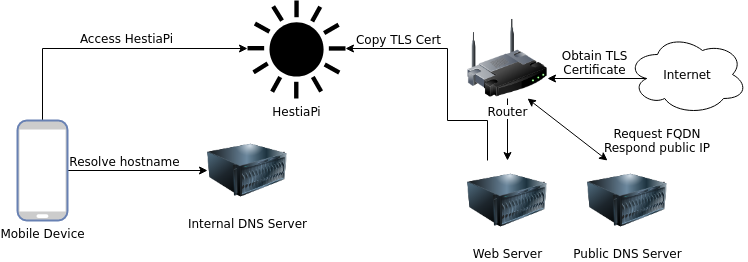
\includegraphics[width=\textwidth]{img/tls_overview.png}
  \caption{Complicated TLS Setup Overview}
  \label{fig:tls-overview}
\end{figure}

\subsubsection{Static IP}
To assign the HestiaPi a static IP address, see section \ref{Static IP}.

\subsubsection{DNS Servers} \label{DNS Servers}
Setting up a DNS server is beyond the scope of this document.  There are many
guides which have been written on the topic, such as
\href{https://www.debuntu.org/how-to-setting-up-a-dns-zone-with-bind9/}{this}.
If you have a bind9 server, adding an entry for the HestiaPi in the internal
DNS server might look like this:

\begin{verbatim}
hestia1                 IN      A       10.1.1.31
\end{verbatim}

The external entry would look the same, but it would be your public IP address
instead of the HestiaPi's internal IP address.  The internal DNS server will
also need to be configured to do recursive DNS lookups.  This is typically
set in \texttt{/etc/bind/named.conf.options} using something like the
following instide the \texttt{options} section:

\begin{verbatim}
allow-recursion { 10.1.1.0/24; localnets; };
allow-query { 10.1.1.0/24; localnets; };
allow-query-cache { 10.1.1.0/24; localnets; };
recursion yes;
\end{verbatim}

For more details on how this works, read
\href{https://www.zytrax.com/books/dns/ch7/queries.html}
{documentation about bind9} or
\href{https://serverfault.com/questions/634546/bind9-proper-recursion-setup/634564#634564}
{this stackoverflow post}.

Updating your computers and mobile devices to point to this name server is best
done at the router.  Instructions for making this change will vary from one
router to the next, but your router's documentation should explain how to change
the nameservers that the DHCP server is assigning.

Once the entry has been added to the nameserver and your computer or device is
using that nameserver, you should be able to access the HestiaPi by name.  In
the example above, the host name would be hestia1 and the domain used in the
linked blog post is debuntu.foo.  This means opening a browser and going to:
\texttt{http://hestia1.debuntu.foo:8080/}

\subsubsection{Obtain TLS certificate}
In order to avoid connecting the HestiaPi to the internet where anyone could
interact with it, this guide shows how to obtain a trusted TLS certificate
using a web server.  At this point it's expected that a public DNS server has
been configured to point to your public IP address (see section
\ref{DNS Servers}).

The next step is to set up a Linux server which will act as the web server.
Once Linux is intalled, you'll need to set up a web server, such as
\href{https://www.nginx.com/resources/wiki/start/topics/tutorials/install/}
{nginx}.  Consult your router's documentation on how to forward port 80 from
your router to the web server.  At this point you should be able to access the
webpage from the internet.  An easy way to test this is to use a mobile phone
or tablet with cell data service.  Disconnect from wifi and attempt to go to
hestia1.example.org and verify there's a web server running.  This verifies
that the DNS, port forwarding and web server are all working correctly.

Follow the \href{https://certbot.eff.org/instructions}{instructions} on how to
use certbot to obtain a TLS certificate.  The
\href{https://letsencrypt.org/docs/}{LetsEncrypt Documentation} is rather
comprehensive and can provide additional context to how their system works.

Once complete, there should be a directory in \texttt{/etc/letsencrypt/live}
for your hostname which contains links to the TLS certificates.

\subsubsection{Configure HestiaPi to use new Certificate}
TODO: Document configuring the HestiaPi to use the newly obtained certificate

